\subsection{Analyse II}
\begin{itemize}
    \item Ist eine Überlappung zwischen Intra- und 
    Interdistanzen gut oder schlecht?
\end{itemize}

Laut Folie 36 der fünften Vorlesung sollte die 
Intradistanzen deutlich kleiner sein als die 
Interdistanzen, ansonsten hat man kein 
funktionierendes System: \glqq Measurement error 
must always be low enough 
to distinguish challenges (intra distance << inter 
distance). Otherwise, the system cannot be used!\grqq

\begin{itemize}
    \item Welche Bedeutung spielt die Größe der 
    Überlappung im Bezug auf die Realisierung einer
    strong-PUF?
\end{itemize}

Die Überlappung sollte gering, sein wenn man eine 
strong-PUF konstruieren möchte. Wie in der Vorlesung
erwähnt wurde zur Folie 36 kann man verschiedene
\textit{Responses} und \textit{Challenges} nicht 
außereinander halten, wenn die Intradistanz groß 
ist. Eine klare Einzigartigkeit der \textit{Responses}
ist erwünscht.


\begin{itemize}
    \item Treffen Sie zu den verschiedenen 
    Plots des Frameworks Aussagen, wie leicht 
    bzw. schwer es ein Angreifer hat, eine 
    Challenge richtig zu raten, wenn er nur 
    die Daten anderer Challenges besitzt. 
    Welche Rolle spielen dabei die 
    verschiedenen Arten des Preprocessings?
\end{itemize}


\verb|No Preprocessing|:
Überlappungs ist hier signifikant. Ein Angreifer hat hier 
mit Abstand die besten Möglichkeiten erfolgreich zu sein.\\


\verb|Euclidean Normalization per Channel|: Intradistanz 
ist gering und fällt streng monoton ab. Die Verteilung der
Interdistanzen hingegen ähnelt einem Hügel mit der Mitte um 
den Wert von etwa 1.8 herum und zu beiden Seiten streng 
monoton abfallend. Der Abstand zwischen den \textit{Peaks} 
beider  Verteilungen ist bisschen weniger als 1,8. Die 
Erfolgsaussichten eines Angreifers sind hier wesentlich 
geringer als oben.\\


\verb|Standardization per Channel|: Hier gibt ein wenig
Überschneidung. Dieses \textit{Preprocessing} bietet
im Vergleich zu den anderen \textit{Preprocessings}
einem Angreifer die besten Chancen.\\


\verb|Standardization per Frequency Bin|: Optisch ähnelt die 
Verteilung der euklidschen Normalisation pro Kanal.
Auffallend ist, dass die Verteilung bei Intradistanz nicht
streng monoton abfallend ist. Der Verteilung bei Interdistanz
erstreckt sich über fast eine Spannweite von 6. Hier hat 
der Angreifer die schlechtesten Chancen.

\begin{figure}[hbt!]
	\centering
		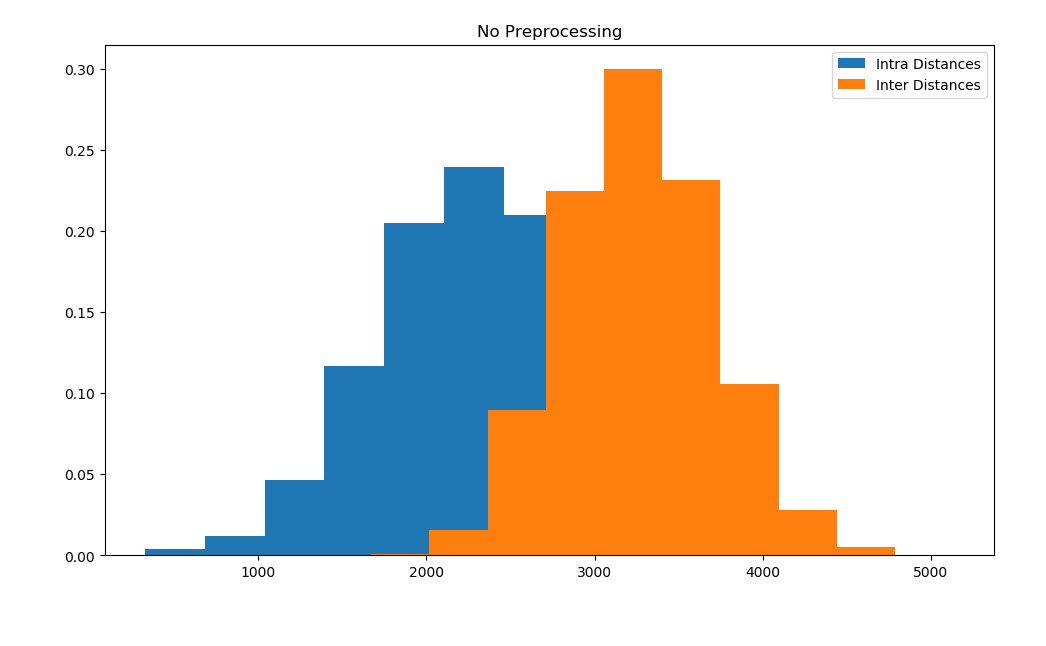
\includegraphics[width=1\textwidth]
		{Bilder/no_preprocessing.png}
		%\caption{no\_preprocessing.png}
		\label{fig:Label1.4.1}
\end{figure}



\begin{figure}[hbt!]
	\centering
		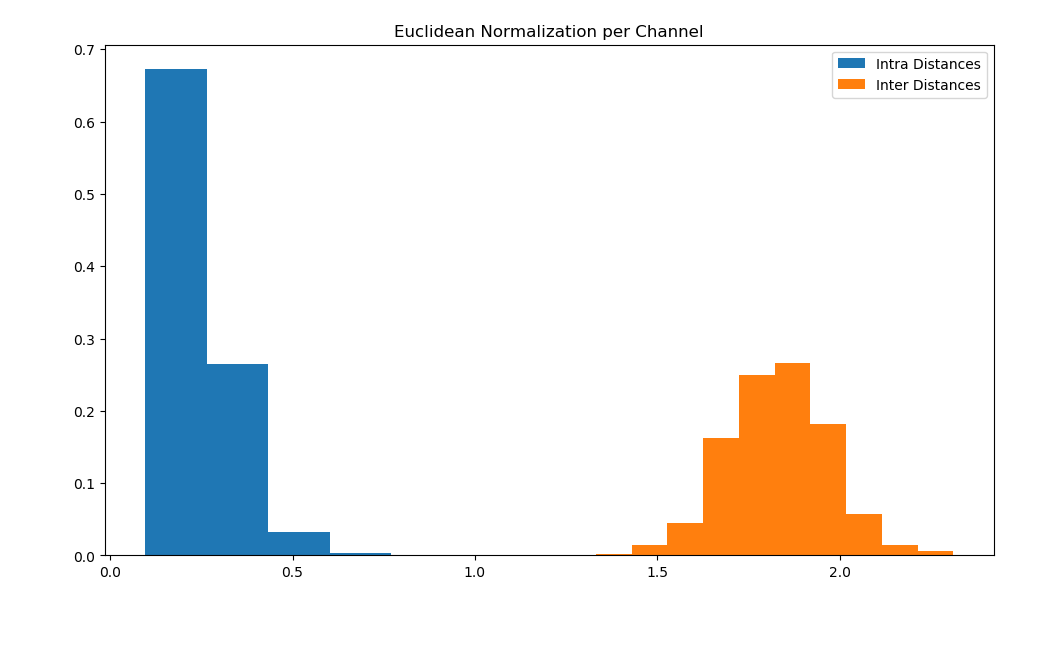
\includegraphics[width=1\textwidth]
		{Bilder/euclid_norm_channel.png}
		%\caption{euclid\_norm\_channel.png}
		\label{fig:Label1.4.2}
\end{figure}



\begin{figure}[hbt!]
	\centering
		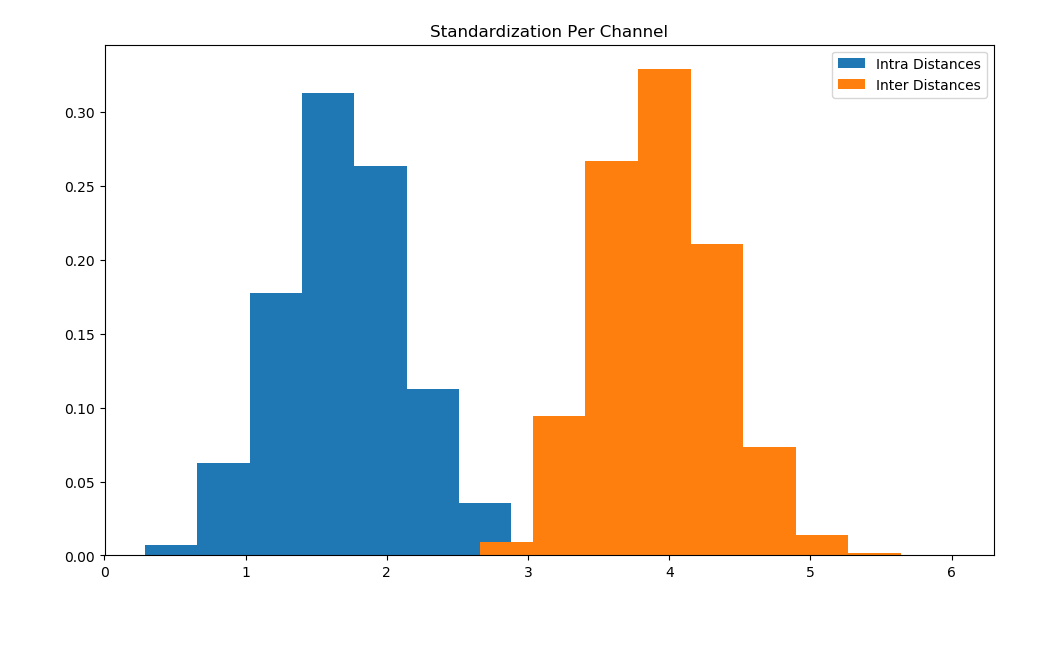
\includegraphics[width=1\textwidth]
		{Bilder/std_channel.png}
		%\caption{std\_channel.png}
		\label{fig:Label1.4.3}
\end{figure}



\begin{figure}[hbt!]
	\centering
		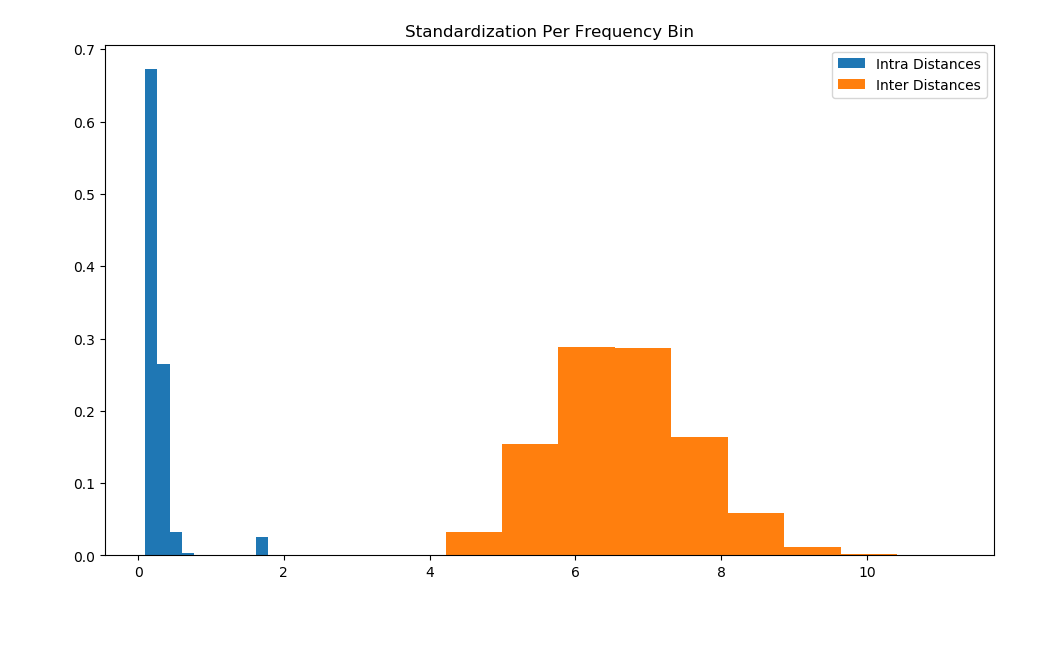
\includegraphics[width=1\textwidth]
		{Bilder/std_freq_bin.png}
		%\caption{std\_freq\_bin.png}
		\label{fig:Label1.4.4}
\end{figure}

 \clearpage